%%% %%%%%%%%%%%%%%%%%%%%%%%%%%%%%%%%%%%%%%%%%%%%%%%%%%%%%%%%%%%%%%%%%%%%%%%%%%%% 

\rawhtml
<a name="foundation_cognitive_neuroscience"></a>
\endrawhtml
\subsectional{Foundation: The Cognitive Neurosciences}

%%% %%%%%%%%%%%%%%%%%%%%%%%%%%%%%%%%%%%%%%%%%%%%%%%%%%%%%%%%%%%%%%%%%%%%%%%%%%%% 

This document is not intended to provide the reader with a short course in cognitive science, artificial intelligence, natural language processing, machine learning, artificial neural networks, or automated code synthesis / automatic inductive programming, and is certainly not intended to cover all these disciplines in any but the most cursory of detail. The primary goal is to explore the possibility of building digital assistants that considerably extend our ability to solve complex engineering problems with a emphasis here on software engineering. A secondary goal is to explain how the field of neuroscience is helping to achieve our primary goal\footnote{%
%
  This particular section concerns the topic of {\urlh{https://en.wikipedia.org/wiki/Knowledge_representation_and_reasoning}{knowledge representation}}~\cite{Brachmanetal2004} as it applies to the programmer's apprentice problem and emphases contributions from the {\urlh{https://en.wikipedia.org/wiki/Cognitive_neuroscience}{cognitive neurosciences}}~\cite{Gazzaniga2009} as they apply to modeling how information is represented and processed in human-inspired cognitive architectures and connectionist models in particular\footnote{%
%
  The phrases {\urlh{https://en.wikipedia.org/wiki/Knowledge_representation_and_reasoning}{Knowledge Representation}}~\cite{Brachmanetal2004} and {\urlh{https://en.wikipedia.org/wiki/Cognitive_neuroscience}{Cognitive Neuroscience}}~\cite{Gazzaniga2009} refer to important long-standing areas of study, each with their respective academic departments, national and international conferences and large numbers of advocates and adepts. Mentioning them both in the same breath could be orthodoxy or heresy depending on the context and the company you keep, but both disciplines \emdash{} it could be argued that each one might be better characterized as a constellation of specialized disciplines\footnote{%
%
  The phrase {\urlh{https://en.wikipedia.org/wiki/Knowledge_representation_and_reasoning}{Knowledge Representation}} seems so dated that it must be back in vogue again. It's interesting to think about the evolution of our thinking about representation as chronicled in the names of major technical conferences relating to artificial intelligence. By 1990, the major national and international AI conferences, including the {\urlh{http://www.aaai.org/Conferences/conferences.php}{National Conference on Artificial Intelligence}} \emdash{} I got roped into co-chairing AAAI-91 held in Anaheim, California \emdash{} and the {\urlh{https://ijcai.org/}{International Joint Conference on Artificial Intelligence}} \emdash{} once again I succumbed to peer pressure and co-chaired IJCAI-99 which was held in Stockholm, Sweden \emdash{} were getting so large and were receiving so many submissions that first satellite and then independent conferences began springing up to cater to special interests including researchers interested in representation.

  For example, Ronald Brachman, Hector Levesque and Raymond Reiter co-chaired the first {\urlh{http://www.kr.org/index.php}{International Conference on Knowledge Representation and Reasoning}} (KR-89) in 1989. Then Usama Fayyad and Ramasamy Uthurusamy chaired the first {\urlh{https://www.aaai.org/Press/Proceedings/kdd95.php}{International Conference on Knowledge Discovery and Data Mining}} (KDD-95) in 1995. More recently Yoshua Bengio and Yann LeCun chaired the first {\urlh{International Conference on Learning Representations}{International Conference on Learning Representations}} (ICLR-13) in 2013. We might extrapolate the trend and imagine Vinod Khosla, Ray Kurzweil, Elon Musk, Peter Thiel and Mark Zuckerberg will co-chair the first {\urlh{https://www.santafe.edu/research/initiatives/interplanetary-project}{Interplanetary Conference on Instantaneous Thought and Infinitely Extensible Memory}} (ITEM-37) in 2037.}
%
\emdash{} have made major contributions to our understanding of intelligence both biological and artificial. Together cognitive neurosciences make up a small but active contingent within the larger population of scientists who consider themselves part of neuroscience including anatomical, behavioral, cellular, cognitive, computational, developmental, genetic, molecular, pharmacological, physiological, psychological and systems neuroscience focusing on neural circuits and their function.}.}.

The fields of cognitive and systems neuroscience are playing an important role in directing and accelerating research on artificial neural network systems. Much of this work predates and helped give rise to the especially exciting work on connectionist models in the 1980s. However, in the nearly 40 intervening years, a great deal of progress has been made, much of it due to improved methods for studying the behavior of awake behaving animal subjects and human beings in particular. Indeed, this work is undergoing a renaissance fueled by even more powerful methods for observing brain activity in human beings in the midst of solving complex cognitive tasks.

The field of automatic programming, after decades of steady, often quite practical research on using symbolic methods \emdash{} much of it originating in labs outside the United States, is seeing a renewed interest in artificial neural networks. It remains to be seen whether artificial neural networks will have a significant impact on code synthesis, however there appear to be opportunities to leverage what we know about both natural and artificial neural networks to make progress, and hybrid systems that combine both connectionist and traditional symbolic methods may have the best chance of pushing the state-of-the-art significantly beyond its present level.

%%% %%%%%%%%%%%%%%%%%%%%%%%%%%%%%%%%%%%%%%%%%%%%%%%%%%%%%%%%%%%%%%%%%%%%%%%%%%%% 

\subsubsectional{Memory}

%%% %%%%%%%%%%%%%%%%%%%%%%%%%%%%%%%%%%%%%%%%%%%%%%%%%%%%%%%%%%%%%%%%%%%%%%%%%%%%

We begin with the problem of how to represent information in memory. In the case of the programmer's apprentice, relevant information includes the type of items that software engineers routinely think about in plying their trade such as algorithms, data structures, interfaces, programs, subroutines and tools such as assemblers, compilers, debuggers, interpreters, parsers and syntax checkers. Then there are the things that programmers generally do not think about explicitly but that concern how they solve problems and organize their thoughts, including, for example, the design strategies we learn in computer science courses such as divide-and-conquer, dynamic-programming and recursion. Finally, there is strategic organizational information of a sort that plays a role in any complex individual or collaborative effort including plans, tasks, subtasks, specifications and requirements.

All of this information has to be encoded in memory and made accessible when required to perform cognitive tasks. Information, whether in a computer or a brain, tends to move around depending on what is to be done with it, and, at least in biological brains, it is constantly changing\footnote{%
%
  The neuroscientist, Moran Cerf, likes to recall an incident that occurred to him when he was young. Cerf enjoyed playing video games but couldn't afford to buy them and so he would go to stores that sold video games and play the demos. He recalls one time in which he started playing a new game and was doing remarkably well after a very short time having reached level III play before being interrupted by a message displayed on the screen that read "Insert coin to play". He then realized that he hadn't been playing the game at all but rather he simply had been moving the joystick and had been imagining \emdash{} indeed he was confident that \emdash{} his moves were causing his meteoric rise in level.

  In hindsight it was clear to him that there were many times in which he had moved the joystick in the wrong direction but had remembered it as being the right direction and having the intended effect of improving his score. His subsequent research focuses on how human memory is susceptible to suggestion to the extent that we often remember what we want to and not what actually happened. Time and memory are intertwined. The former we experience as being incongruously mutable \emdash{} an hour can seem infinitesimally short and a second interminably long, while the latter seems to us incontrovertibly fixed and yet neuroscience tells us that memories are subject to fantasy and random happenstance. 

  If you're interested Moran Cerf's research, check out this YouTube{\urlh{https://www.youtube.com/watch?v=EVj3sU37gdI}{}{video}} of Cerf speaking at Talks at Google in which he "describes his lab's work studying the brains of humans using unique tools to eavesdrop on the activity of individual cells of patients undergoing brain surgery while they are awake and behaving. He discusses how the work sheds light on the ways our brain processes information, and reflects on what it tells us about how we create the complex narrative we call 'us'."}.
%
In biological brains, it is difficult if not impossible to think about something without changing it. In building systems inspired by biological brains we have somewhat more control over such changes, but control comes at a cost. We make no distinction between concrete and abstract thoughts \emdash{} all thoughts are abstract whether they represent atoms or bits. We will on occasion refer to memories as being short- or long-term but the distinction doesn't begin to address real issues. When we talk about episodic memory, it may seem that we are referring to some sort of permanent or archival memory, but that's not the case.

Since this document is more condensed precis than unabridged thesis, we need some way of navigating the huge space of ideas relating to biological and artificial brains as they pertain to building digital assistants and automatic programming. I'll begin by pointing out that language, programs and plans are all usefully thought of as having hierarchical, recursive structure. It also makes sense to think of brains as being organized as such~\cite{Ballard2015,Kurzweil2012,DeanAMAI-06,GeorgeandHawkinsIJCNN-05,DeanAAAI-05,Hawkins04}, and the human brain apparently employs hierarchical models to make sense of the world in which it evolved. 

To the untutored mind, the world is essentially flat. We impose hierarchical structure to make understanding it more tractable. We ingest sequences of observations as input and execute sequences of actions as output. What goes on between is complicated. Rather than immediately focusing on how biological and artificial brains learn and apply hierarchical models, we start by considering the simpler problem of how we might represent a {\it{subroutine}}, the smallest fungible unit of activity for our purposes. Subroutines can be used to kick a soccer ball or implement simple program transformations in a neural-network architecture.

%%% %%%%%%%%%%%%%%%%%%%%%%%%%%%%%%%%%%%%%%%%%%%%%%%%%%%%%%%%%%%%%%%%%%%%%%%%%%%%

\rawhtml
<a name="convention_and_abbreviation_index"></a>
\endrawhtml
The following assumes familiarity with artificial neural networks\footnote{%
%
  The jargon of modern (deep) neural networks is like the argot of a new Freemasonry that has hardly begun to lay the foundations for the restoration of the connectionist temple. Terms like attention, consciousness, imagination, rewards and reinforcement get bandied about as if deeply descriptive of the architectures they are invoked to describe. The odd thing is that often they reveal more than they obfuscate. Even so, the learning curve is steep, and the mountain is constantly shifting.}. 
%
We begin with the simplifying assumption that subroutines can be represented as tuples consisting of a set of operands represented as high-dimensional embedding vectors, a weight matrix representing the transformation and a product vector space in which to embed the result. In applying this idea to program transformations, assume that each operand corresponds to the embedding of an abstract-syntax-tree representation of a code fragment, w.l.o.g., any non-terminal node in the AST of a syntactically well-formed program. In the remainder of this section and the next, we use the following abstractions and abbreviations:
%
\begin{itemize}
%
\item {\it{prefrontal cortex}} (PFC) including attention, conscious access, reward-based-learning and executive control~\cite{WangetalNATURE-NEUROSCIENCE-18,KrieteetalPNAS-13};
%
\item {\it{entorhinal-hippocampal complex}} (EHC) in its role as primary interface between the hippocampus and neocortex~\cite{OReillyetalCS-15,OReillySCIENCE-06};
%
\item {\it{global workspace}} (GW) broadly distributed cortical circuits connected through long-range excitatory axons\footnote{%
%
    Dehaene~\etal{DehaeneetalPNAS-98} distinguish two main computational spaces within the brain: "The first is a {\it{processing network}}, composed of a set of parallel, distributed and functionally specialized processors or modular sub-systems ranging from primary sensory processors (such as area V1) or unimodal processors (such as area V4), which combine multiple inputs within a given sensory modality, up to heteromodal processors (such as the visuo-tactile neurons in area LIP) that extract highly processed categorical or semantic information. Each processor is subsumed by topologically distinct cortical domains with highly-specific local or medium-range connections that {\it{encapsulate}} information relevant to its function.

    The second computational space is a {\it{global workspace}}, consisting of a distributed set of cortical neurons characterized by their ability to receive from and send back to homologous neurons in other cortical areas horizontal projections through long-range excitatory axons (which may impinge on either excitatory or inhibitory neurons). Our view is that this population of neurons does not belong to a distinct set of {\it{cardinal}} brain areas but, rather, is distributed among brain areas in variable proportions."}~\cite{DehaeneetalPNAS-98,Baars1988};
%
\item {\it{basal ganglia}} (BG) for its role in action selection and dynamic gating to direct input to the prefrontal cortex\cite{OReillyetalLEABRA-16,KrieteetalPNAS-13};
% 
\item {\it{semantic memory system}} (SMS) including areas of the brain responsible for mathematical and abstract thought~\cite{Tulving1972,BinderandDesaiTiCS-11};
%
\item {\it{episodic memory system}} (EMS) including episodic memory management and memory-based parameter adaptation~\cite{SprechmannetalICLR-18,PritzeletalICML-17};
%
\item {\it{differentiable neural computer}} (DNC) as the interface to the integrated development environment prostheses~\cite{GravesetalNATURE-16,GravesetalCoRR-14};
%
\item {\it{abstract syntax-tree}} (AST) is a representation of the abstract syntactic structure of a source-code program\footnote{%
%
  Here is the abstract syntax tree for {\urlh{https://en.wikipedia.org/wiki/Euclidean_algorithm}{Euclid's algorithm}} which is an efficient method for computing the greatest common divisor (GCD) of two numbers:
  % 
  \begin{center}
    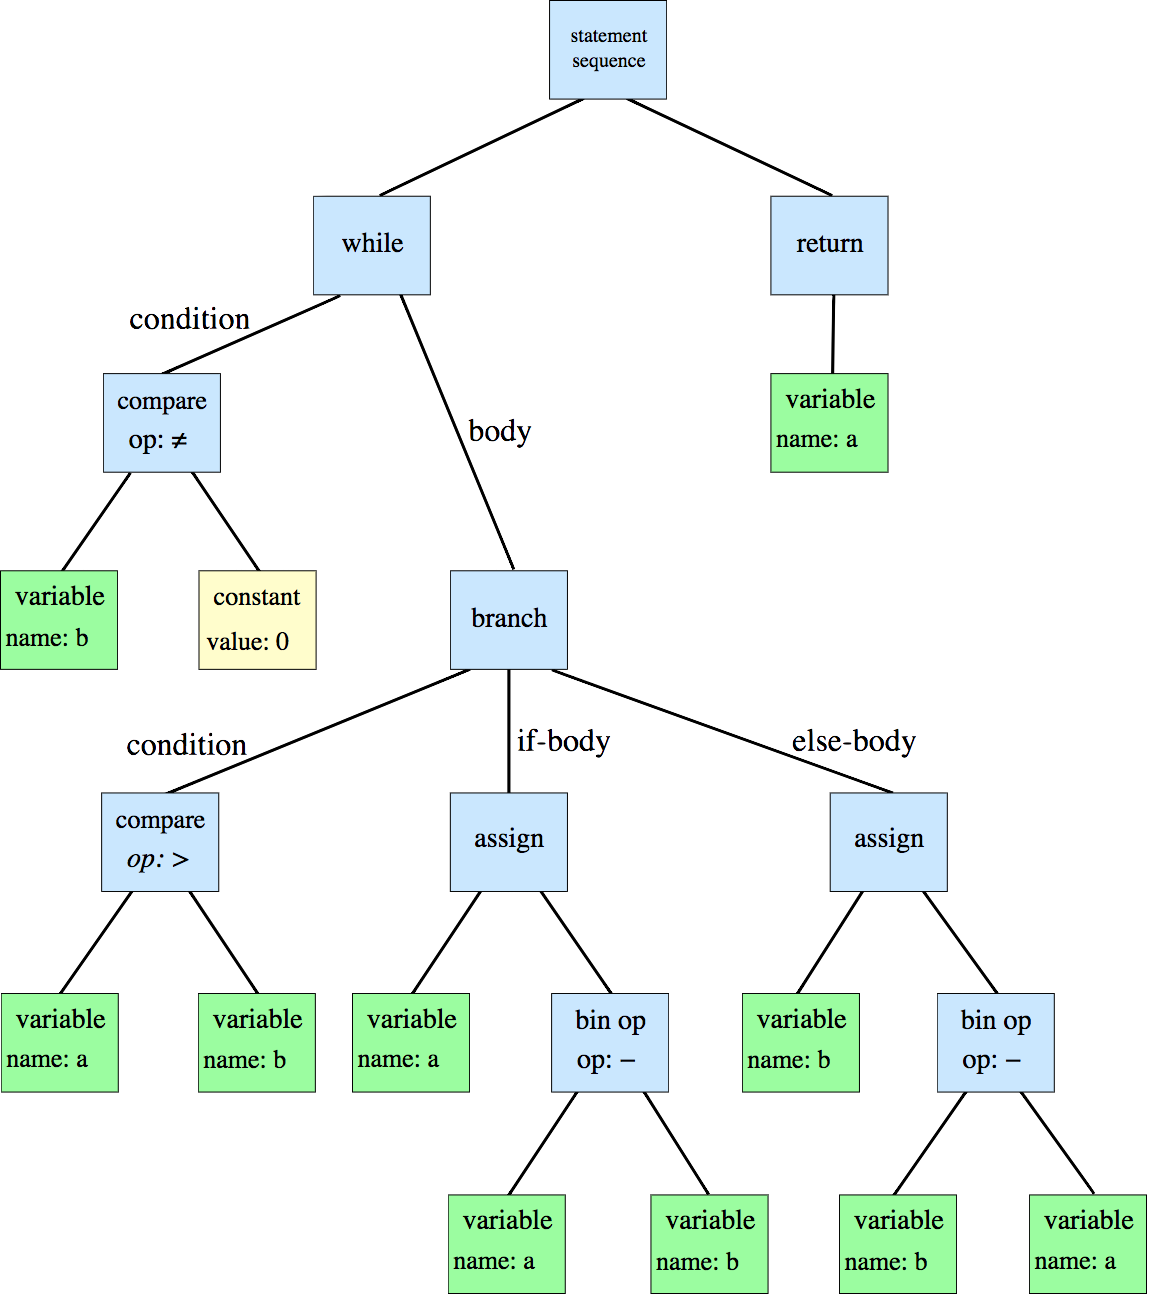
\includegraphics[width=6.0in]{./figures/Euclids_Greatest_Common_Divisor_Method.png}
  \end{center}}~\cite{DevlinetalICLR-18,WangetalCoRR-17};
% 
\end{itemize}

The second introductory lecture ({\urlh{https://web.stanford.edu/class/cs379c/calendar_invited_talks/lectures/04/05/slides/index.html}{HTML}}) for the Stanford {\urlh{https://web.stanford.edu/class/cs379c/}{course}} associated with this document provides a high-level overview of the relevant research in cognitive and systems neuroscience. Annotations of the form "Slide \#" link to relevant slides in the introductory lecture. For example {{\urlh{https://web.stanford.edu/class/cs379c/calendar_invited_talks/lectures/04/05/slides/index.html#CS379C_INTRODUCTORY_LECTURE_2_SLIDE_02}{Slide~2}}} covers the key anatomical landmarks in the human brain mentioned in this document. While the material in the remainder of this section refers to work in cognitive and systems neuroscience, the discussion here emphasizes applications of what we've learned from neuroscience, and so the interested reader is encouraged to at least skim the above-linked lecture notes.

%%% %%%%%%%%%%%%%%%%%%%%%%%%%%%%%%%%%%%%%%%%%%%%%%%%%%%%%%%%%%%%%%%%%%%%%%%%%%%%

Referring to the abstractions and abbreviations introduced in the previous section, reading a program from {\tt{STDIO}} \emdash{} the analog of a human programmer reading a program displayed on a monitor \emdash{} will result in \emdash{} at least \emdash{} two different internal representations of the resulting AST: an embedding vector in the SMS and a key-value representation in the DNC. The former allows us manipulate programs and program fragments as fully-differentiable representations within distributed models. The latter allows us to modify, execute and share code in a human-accessible format, fully compatible with our software-development toolchain.

Following~\cite{PritzeletalICML-17}, we assume EMS consists of initial-state-action-reward-next-state tuples of the form $(s_{t},\;a_{t},\;r_{t},\;s_{t+1})$. State representations $s_{t}$ have to be detailed enough to reconstruct the context in which the action is performed and yet concise enough to be practical. Suppose the PFC directs the activation of selected circuits in the SMS via the global workspace (GW) \emdash{} see Slides~{{\urlh{https://web.stanford.edu/class/cs379c/calendar_invited_talks/lectures/04/05/slides/index.html#CS379C_INTRODUCTORY_LECTURE_2_SLIDE_03}{3}}} and~{{\urlh{https://web.stanford.edu/class/cs379c/calendar_invited_talks/lectures/04/05/slides/index.html#CS379C_INTRODUCTORY_LECTURE_2_SLIDE_05}{5}}} \emdash{} in accord with Dehaene~\etal{}~\cite{DehaeneetalSCIENCE-17,Dehaene2014} assuming a prior that generates low-dimensional thought vectors~\cite{BengioCoRR-17}. The state representation $s_{t}$ encodes the attentional state that served to identify representations in SMS relevant to $a_{t}$ allowing the EHC to produce the resulting state $s_{t+1}$. Given $s_{t}$ we can reproduce the activity recorded in the EMS, and, in principle, incorporate multiple steps and contingencies in a policy constituting a specialized program-synthesis or program-repair subroutine.

Such subroutines would include repairing a program in which a variable is introduced but not initialized, or when it is initialized but ambiguously typed or scoped. As another example, a variable is initialized as {\tt{VOID}} and subsequently assigned an integer value in some but not all branches of a conditional statement. Other examples of repair routines include problems with the use of comparison operators, e.g., conditional branches both with \hmleq{}, the {\tt{is}} operator is used instead of {\tt{is not}}, or vice versa, confusion involving {\tt{A is not None}}, {\tt{A not None}} and {\tt{A != None}}, and problems involving class methods, e.g., when {\tt{self}} accessor is missing from a variable, e.g., {\tt{mode = 'manual'}} instead of {\tt{self.mode = 'manual'}}~\cite{ShinetalICLR-18b,DevlinetalICLR-18,WangetalCoRR-17}.

Attentional machinery in the prefrontal cortex (PFC) populates the (GW) by activating circuits relevant to the current input and internal state, including that of the DNC and any ongoing activity in (SMS) circuits produced by previous top-down attention and bottom-up sensory processing. The PFC in its role as executive arbiter identifies operators in the form of policy subroutines and then enlists the EHC to \emdash{} using terminology adapted from Von Neumann machines \emdash{} to load registers in short-term memory and perform operations by using fast weights to transform the contents of the loaded registers into product representations that can either be fed to associative embeddings, temporarily stored in other registers or used to modify the contents of the DNC thereby altering the AST representation of the target code and updating the display to provide feedback to the human programmer.

The primate cortex appears to be tiled with columnar structures referred to as {\it{cortical columns}}. Some neuroscientists believe that all of these columns compute the same basic function. However, there is considerable variation in cell type, thickness of the cortical layers, and the size of the dendritic arbors to question this hypothesis. The prefrontal cortex is populated with a type of neuron, called a {\it{spindle neuron}}, similar in some respects to the {\it{pyramidal cells}} found throughout the cortex, that allow rapid communication across the large brains of great apes, elephants, and cetaceans. Although rare in comparison to other neurons, spindle neurons are abundant and quite large in humans and apparently play an important role in consciousness and attentional networks \emdash{} see {{\urlh{https://web.stanford.edu/class/cs379c/calendar_invited_talks/lectures/04/05/slides/index.html#CS379C_INTRODUCTORY_LECTURE_2_SLIDE_04}{Slide~4}}}.

The corresponding artificial neural network architecture for the programmer's apprentice application consists of a hierarchy of specialized networks with a relatively dense collection of feedforward and feedback connections that enable recurrent state, attentional focus and the management of specialized memory systems that persists across different temporal scales \emdash{} see {{\urlh{https://web.stanford.edu/class/cs379c/calendar_invited_talks/lectures/04/05/slides/index.html#CS379C_INTRODUCTORY_LECTURE_2_SLIDE_06}{Slide~6}}}. Individual networks are specialized to serve different types of representation, employing convolutional networks, gated-feedback recurrent networks and specialized embedding models. All of these networks are distributed representations that encode information in high-dimensional vector spaces such that different dimensions can be trained to represent different features allowing attentional mechanisms to emphasize or modify encodings so as to alter their meaning.

These attentional networks are connected to regions throughout the cortex and are trained via reinforcement learning to recognize events worth attending to according to the learned value function. Using extensive networks of connections \emdash{} both incoming and outgoing, attentional networks are able to create a composite representation of the current situation that can serve a wide range of executive cognitive functions, including decision making and imagining possible futures. The basic idea of a neural network trained to attend to relevant parts of the input is key to a number of the systems that we'll be looking at.

To understand attentional networks, think about an encoder-decoder network for machine translation. As the encoder digests each word in the sequence of words that constitute the input sentence, it produces a representation \emdash{} Geoff Hinton refers to these as {\it{thought clouds}} in analogy to the iconic clouds that you see in comic strips \emdash{} of the sentence fragment or {\it{prefix}} that it has seen so far. Because the sentence is ingested one word at a time \emdash{} generally proceeding from left to right \emdash{} the resulting thought cloud will tend to emphasize the meaning of the most recently ingested words in each prefix. You could encode the entire input sentence and then pass the resulting representation on to the decoder, but earlier words in the sentence will receive less attention that later words. Alternatively, you could introduce a new network layer that takes as input encodings of all the sentence prefixes seen so far and trains the new layer \emdash{} thereby taking advantage of the power of gradient descent \emdash{} to produce a composite representation that emphasizes those parts of the input that are most relevant in decoding / generating the next word in the output.

The programmer's apprentice is implemented as an instance of an hierarchical neural network architecture. It has a variety of conventional inputs that include speech and vision, as well as output modalities including speech and text. In these respects, it operates like most existing commercial personal assistants \emdash{} see {{\urlh{https://web.stanford.edu/class/cs379c/calendar_invited_talks/lectures/04/05/slides/index.html#CS379C_INTRODUCTORY_LECTURE_2_SLIDE_07}{Slide~7}}}. It differs substantially, however, in terms of the way in which the apprentice interacts with the programmer. It is useful to think of the programmer and apprentice as pair programming, with the caveat that the programmer is in charge, knows more than the apprentice does \emdash{} at least initially, and is invested in training the apprentice to become a competent software engineer. One aspect of their joint attention is manifest in the fact that they share a browser window. The programmer interacts with the browser in a conventional manner while the apprentice interacts with it as though it is part of its body directly reading and manipulating the HTML using the browser API. The browser serves both programmer and apprentice as an encyclopedic source of useful knowledge as well as another mode of interaction and teaching.

The spatial relationships among the ganglion cells in the retina are preserved in the activity of neurons found in the primary visual \emdash{} or {\it{striate}} \emdash{} cortex. Most sensory and motor areas maintain similar modality-specific topographic relationships. Shown {{\urlh{https://web.stanford.edu/class/cs379c/calendar_invited_talks/lectures/04/05/slides/index.html#CS379C_INTRODUCTORY_LECTURE_2_SLIDE_10}{here}}}, for example, are Wilder Penfield's famous motor and somatosensory {\urlh{https://en.wikipedia.org/wiki/Cortical_homunculus}{homunculi}} depicting the areas and proportions of the human brain dedicated to processing motor and sensory functions. Scientists have observed that the area devoted to the hands tend to be larger among pianists, while the relevant areas in the brains of amputees typically become significantly smaller \emdash{} see {{\urlh{https://web.stanford.edu/class/cs379c/calendar_invited_talks/lectures/04/05/slides/index.html#CS379C_INTRODUCTORY_LECTURE_2_SLIDE_10}{Slide~10}}}.

We imagine the programmer's apprentice with a body part consisting of an instrumented {\it{integrated development environment}} (IDE). Alternatively you might think of it as a prosthetic device. It is not, however, something that you can simply remove or replace with an alternative device outfitted with a different interface or supporting different functions and expect it to immediately respond to your attempts to control it \emdash{} it is not a plug-and-play device. Like the legs you were born with or the prosthesis replacing an amputee's severed arm, you have to learn how to use these devices. Architecturally, the apprentice's prosthetic IDE is an instance of a {\it{differentiable neural computer}} (DNC) introduced by Alex Graves and his colleagues at DeepMind. The assistant combined with its prosthetic IDE is neural network that can read from and write to an external memory matrix, combining the characteristics of a random-access memory and set of memory-mapped device drivers and programmable interrupt controllers. The interface supports a fixed number of commands and channels that provide feedback. You can think of it as roughly similar to an Atari game console \emdash{} see {{\urlh{https://web.stanford.edu/class/cs379c/calendar_invited_talks/lectures/04/05/slides/index.html#CS379C_INTRODUCTORY_LECTURE_2_SLIDE_11}{Slide~11}}}.

What is left out of this account so far includes how we might take advantage of semantics in the form of executing code and examining traces in order to better understand the consequences of the changes just made. Presumably, wrapping a code fragment in a function and executing the function with different input to examine changes in the state variables could be used as a distal reinforcement signal providing intermediate rewards useful in debugging subroutines. As pointed out earlier, subroutines designed to modify code are likely to involve many conditional choices and so it is important for subroutine policies to be highly conditioned on the status of specific state variables. Indeed a technique such as model-based parameter adaptation may be perfectly suited to providing such context-sensitive adaptations.

Perhaps this next observation seems obvious, but it is worth keeping in mind that the human brain does a great deal of (parallel) processing that never rises to the level of conscious attention. The executive control systems in the prefrontal cortex don't have micromanage everything. Every thought corresponds to a pattern of activity in one or more neural circuits in the brain or beyond in the peripheral nervous system. One pattern of activity inevitably leads to another in the same or another set of neurons. For example, patterns of activity that begin in the sensory cortex can lead to patterns of activity in the motor cortex and can have consequences elsewhere in the brain, e.g., in the cerebellar cortex resulting in speech, or external to the central nervous system as in the case of neurons that propagate through the peripheral nervous system causing muscles to contract and extend thereby making your limbs and torso move. 

Every new observation, every act of creating a new thought or revisiting an old one produces even more activity in the brain resulting in new thoughts some of which are ignored as their reverberations weaken and die and others that spawn new thoughts and proliferate under the influence of reentrant production of activity and the active encouragement of conscious attention in a perpetually self reinforcing, reimagining and self-analyzing cycle of recurrent activity. Meta-reinforcement learning supports the sort of diverse activity one might expect from a system that selects activity to attend to and then makes available in the global workspace for ready access by other systems. Sustaining a collection of such activated circuits would help to provide a context, serve to maintain a stack of policies, guide switching between them, support caching partial results for later use, reconstructing necessary state as needed when restoring policy after a recursive descent.

When you think of building systems that can develop new algorithms it is instructive the think about the simple case of learning to sort lists from input-output pairs. The bubble sort algorithm is generally regarded as the easiest to come up with, but even then it is easier if you start with simple I/O pairs like $[A,\;B] \hmrarr{} [A,\;B], [B,\;A] \hmrarr{} [A,\;B]$ and work up to longer lists \emdash{} referred to as curriculum learning~\cite{BengioetalICML-09}. As Dan Abolafia pointed out in his class {\urlh{https://web.stanford.edu/class/cs379c/calendar_invited_talks/lectures/04/24/index.html}{presentation}}, it is relative easy to learn to sort lists of length no more than $n$, but substantially more difficult to learn an algorithm that works for lists of arbitrary length, without the ability to construct a simple inductive proof of correctness. Logic and basic theorem proving are certainly important in learning to write programs. You might want to look at the Coq proof assistant\footnote{%
%
  {\urlh{https://en.wikipedia.org/wiki/Coq}{Coq}} is a formal proof management system that "provides a formal language to write mathematical definitions, executable algorithms and theorems together with an environment for semi-interactive development of machine-checked proofs" \emdash{} excerpted from Mike Nahas' {\urlh{https://coq.inria.fr/tutorial-nahas}{tutorial}}. The Coq formal language is also a programming language. It was developed by and named after its inventor, Thierry Coquand, and employed by Georges Gonthier and Benjamin Werner to create a new proof of the {\urlh{https://en.wikipedia.org/wiki/Four_color_theorem}{Four Color Theorem}} first proved by Kenneth Appel and Wolfgang Haken using a combination of human and computer theorem proving techniques.} for a glimpse at the future of algorithm development.

%%% %%%%%%%%%%%%%%%%%%%%%%%%%%%%%%%%%%%%%%%%%%%%%%%%%%%%%%%%%%%%%%%%%%%%%%%%%%%% 

\setcounter{figure}{0}

%%% %%%%%%%%%%%%%%%%%%%%%%%%%%%%%%%%%%%%%%%%%%%%%%%%%%%%%%%%%%%%%%%%%%%%%%%%%%%% 

%%% Figure~{\urlh{#fig_Integrated_Architecture_Integrated_Figure}{1}}
\rawhtml
<a name="fig_Integrated_Architecture_Integrated_Figure"></a>
\endrawhtml
\begin{figure}
%
  \hrule{}
%
  \begin{center}
    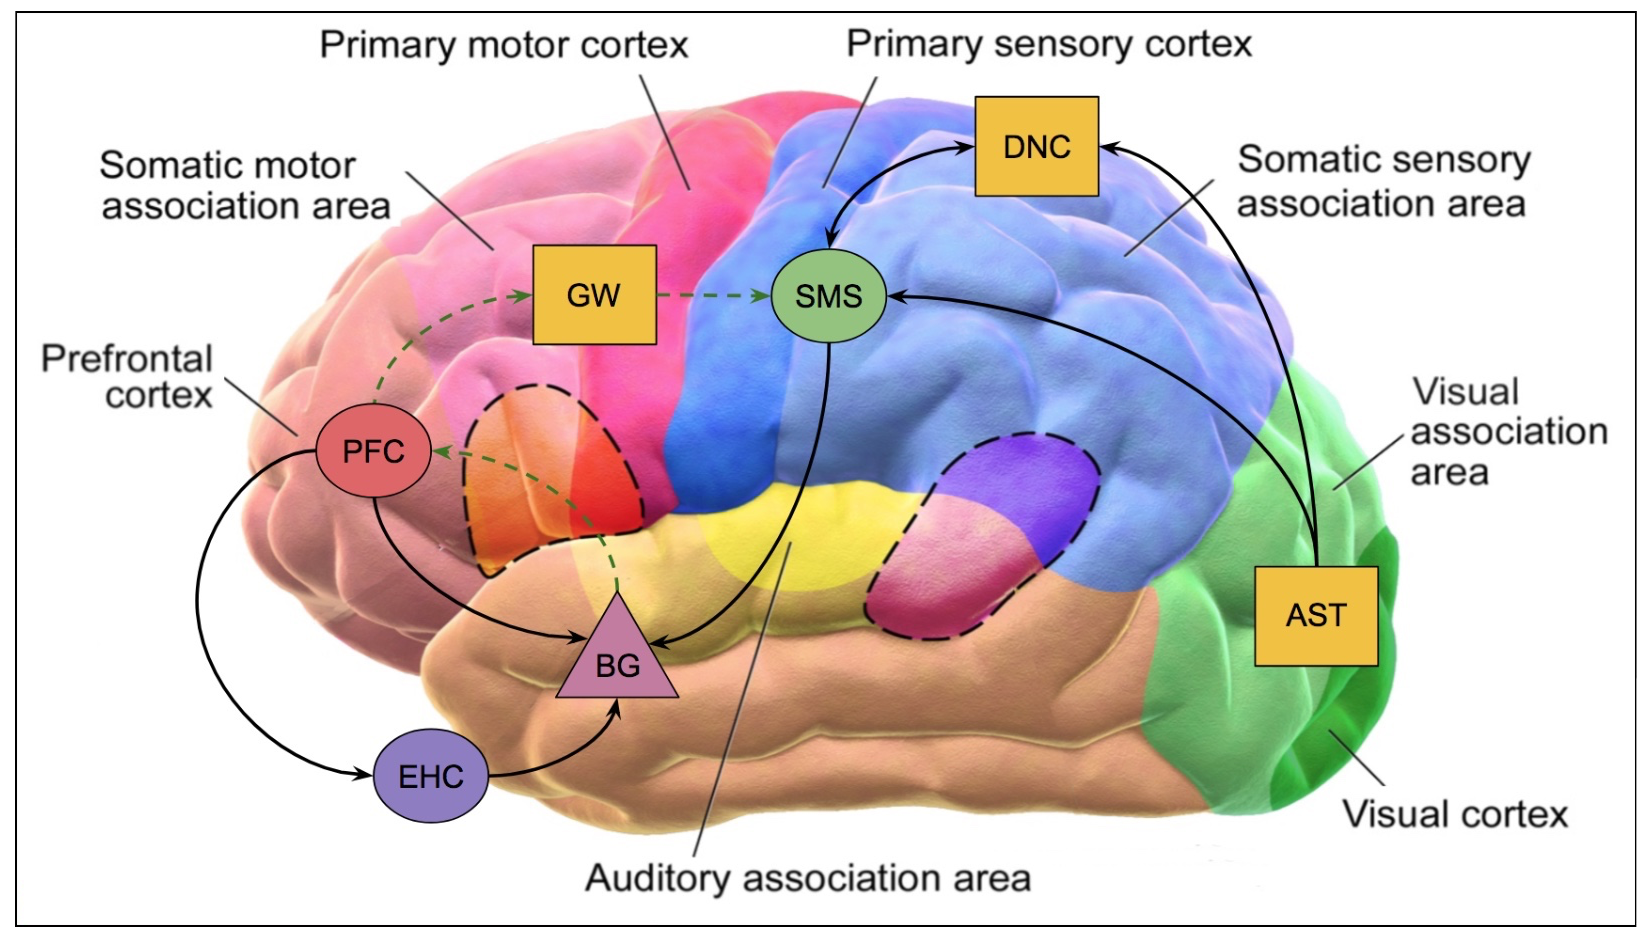
\includegraphics[width=10.0in]{./figures/Integrated_Architecture_Integrated_Figure.jpg}
  \end{center}
%
  \caption{This figure highlights the primary architectural components mentioned in the main text superimposed over an anatomical rendering of the human brain identifying related cortical and sub-cortical landmarks. The triangle and three ovals and match the shape and color conventions employed in O'Reilly~\cite{OReillySCIENCE-06} where you will find a substantially more detailed explanation of the underlying biological model. The three gold square shapes denote abstract architectural structures and not anatomical features. The acronyms are expanded and explained {\urlh{#convention_and_abbreviation_index}{here}}.}
%
  \hrule{}
%
\end{figure}

%%% %%%%%%%%%%%%%%%%%%%%%%%%%%%%%%%%%%%%%%%%%%%%%%%%%%%%%%%%%%%%%%%%%%%%%%%%%%%% 

Figure~{\urlh{#fig_Integrated_Architecture_Integrated_Figure}{1}} shows a diagram of the human brain overlaid with a simplified architectural drawing. The box shapes represent abstract systems and the oval and triangular shapes represent anatomical features for which we can supply computational models. For example, the box labeled GW represents the global workspace which performs a particular function in the architecture, but actually spans a good portion of the neocortex. Whereas the triangle labeled BG represents a group of subcortical nuclei called the basal ganglia situated at the base of the forebrain.

The box labeled AST represents a form of sensory input corresponding to the ingestion of abstract syntax trees representing code fragments. The oval labeled SMS represents semantic memory and the box labeled DNC corresponds to a differentiable neural computer. When the system ingests a new program fragment the resulting AST is encoded in the SMS as an embedding vector and simultaneously as a set of key-value pairs in the DNC. Here we think of the DNC as a body part or external prosthesis with corresponding maps in the somatosensory and motor cortex that enable reading and writing respectively \emdash{} see Slides~{{\urlh{https://web.stanford.edu/class/cs379c/calendar_invited_talks/lectures/04/05/slides/index.html#CS379C_INTRODUCTORY_LECTURE_2_SLIDE_10}{10}}} and~{{\urlh{https://web.stanford.edu/class/cs379c/calendar_invited_talks/lectures/04/05/slides/index.html#CS379C_INTRODUCTORY_LECTURE_2_SLIDE_11}{11}}} mentioned earlier.

Our explanation of the architecture proceeds top down, as it were, with a discussion of executive function in the prefrontal cortex. The GW provides two-way connection between structures in the prefrontal cortex and homologous structures of a roughly semantic character throughout the rest of neocortex thereby enabling the PFC to listen in on diverse circuits in the neocortex and select a subset of such circuits for attention. Stanislas Dehaene describes this process as one of the primary functions of consciousness, but we need not commit ourselves to such interpretation here.

Not only does the PFC selectively activate circuits but it can also maintain the activity such circuits indefinitely as constituents of working memory. Since this capability is limited by the capacity of the PFC, the content of working memory is limited and adding new constituents may curtail the activation of existing constituents. In practice, we intend to model this capability using meta-reinforcement learning~\cite{WangetalNATURE-NEUROSCIENCE-18} (MRL) in which the MRL system relies on the GW network to sample, evaluate and select constitutuent circuits guided by a suitable prior~\cite{BengioCoRR-17} and past experience and then maintain their activity by a combination of memory networks~\cite{WestonetalCoRR-14} and fast weights~\cite{BaetalCoRR-16}. 

%%% %%%%%%%%%%%%%%%%%%%%%%%%%%%%%%%%%%%%%%%%%%%%%%%%%%%%%%%%%%%%%%%%%%%%%%%%%%%% 

Meta-reinforcement learning serves a second complementary role in the PFC related to executive function. We will refer to the first role as MRL-A for "attention" and the second as MRL-P for "planning". MRL-A is trained to focus attention on relevant new sensory input and new interpretations of and associations among prior perceptions and thoughts. MRL-P is trained to capitalize on and respond to opportunities made available by new and existing constituents in working memory. Essentially MRL-P is responsible for the scheduling and deployment of plans relevant to recognized opportunities to act. These plans are realized as policies trained by reinforcement learning from traces of past experience or constructed on the fly in response to unexpected / unfamiliar contingencies by recovering and reimagining past activities recovered from episodic memory \emdash{} see~{{\urlh{https://web.stanford.edu/class/cs379c/calendar_invited_talks/lectures/04/05/slides/index.html#CS379C_INTRODUCTORY_LECTURE_2_SLIDE_13}{Slide~13}}}.

MRL-A and MRL-P could be implemented as a single policy, but it is simpler to think of them as two coupled systems, one responsible for focusing attention by constantly assessing changes in (neural) activity throughout the global workspace, and a second responsible for overseeing the execution of plans in responding to new opportunities to solve problems. MRL-A is as a relatively straightforward reinforcement learning system independently performing its task largely a function of whatever neural activity is going on in the GW, its attentional network and the prior baked into its reward function. MRL-P could be implemented along the lines of the Imagination-Augmented Agent (I2A) architecture~\cite{WeberetalCoRR-17} or the related Imagination-Based Optimization~\cite{HamricketalCoRR-17} and Imagination-Based Planning~\cite{PascanuetalCoRR-17} systems.

%%% %%%%%%%%%%%%%%%%%%%%%%%%%%%%%%%%%%%%%%%%%%%%%%%%%%%%%%%%%%%%%%%%%%%%%%%%%%%%

The remaining parts of the architecture involve the interplay between the PFC and the semantic and episodic memory systems as facilitated by the basal ganglia and hippocampus. If we had a policy pre-trained for every possible contingency, we would be nearly done \emdash{} let MRL-A draw attention to relevant internal and external activity and then design a simple just-in-time greedy scheduler that picks the policy with the highest reward given the state vector corresponding to the current content of working memory. Unfortunately, the life of an apprentice programmer is not nearly so simple. The apprentice might listen to advice from a human programmer or watch someone solve a novel coding problem or repair a buggy program. Alternatively, it may be relatively simple to adapt an existing policy to work in the present circumstances. However, making progress on harder problems will depend on expert feedback or having an existing reward function that generalizes to the problem at hand. 

The hippocampus is perhaps best known for its role in supporting spatial reasoning. A type of pyramidal neuron called a {\it{place cell}} has been shown to become active when an experimental animal enters an area of a maze that it has visited before. However, the hippocampus plays a much larger role in memory by representing not just the "where" of experience but also the "when". The manner in which we employ short- and long-term memory is very different. We might construct a representation of our current situation in short-term memory, drawing upon our long-term memory to provide detail. 

The two memory systems are said to be complementary in that they serve different purposes, one provides an archival record of the past while the other serves as a scratchpad for planning purposes. In retrieving a memory there is a danger that we corrupt the long-term memory in the process of subsequent planning. This isn't simply an academic question, it is at the heart of how we learn from the past and employ what we've learned to think about the future. Our subtle memory systems enable us to imagine solutions to problems that humans have never faced, and account for a good deal of our incredible adaptivity. In several lectures, we will explore architectures that support such flexibility \emdash{} see {{\urlh{https://web.stanford.edu/class/cs379c/calendar_invited_talks/lectures/04/05/slides/index.html#CS379C_INTRODUCTORY_LECTURE_2_SLIDE_14}{Slide~14}}}.

%%% %%%%%%%%%%%%%%%%%%%%%%%%%%%%%%%%%%%%%%%%%%%%%%%%%%%%%%%%%%%%%%%%%%%%%%%%%%%%

\subsubsectional{Actions}

%%% %%%%%%%%%%%%%%%%%%%%%%%%%%%%%%%%%%%%%%%%%%%%%%%%%%%%%%%%%%%%%%%%%%%%%%%%%%%%

The basal ganglia in cognitive models such as the one described by Randall O'Reilly's in his {\urlh{https://web.stanford.edu/class/cs379c/calendar_invited_talks/lectures/04/12/index.html}{presentation}} in class, play a central role in action selection. This seems like a good opportunity to review how actions are represented in deep-neural-network implementations of reinforcement learning. Returning to our default representation for the simplest sort of episodic memory, $(s_{t},\;a_{t},\;r_{t},\;s_{t+1})$, it’s easy to think of a state $s$ as a vector $s \hmisin{} \hmreals{}^{n}$ and a reward $r$ as a scalar value, $r \hmisin{} \hmreals{}$, but how are actions represented?

Most approaches to deep reinforcement learning employ a tabular model of the policy implying a finite \emdash{} and generally rather small \emdash{} repertoire of actions. For example, most of the experiments described in Wayne~\etal{}~\cite{WayneetalCoRR-18} (MERLIN) six-dimensional one-hot binary vector that maps a set of six actions: move forward, move backward, rotate left with rotation rate of 30, rotate right with rotation rate of 30, move forward and turn left, move forward and turn right. The action space for the grid-world problems described in Rabinowitz~\etal{}~\cite{RabinowitzetalCoRR-18} (ToMnets) consists of four movement actions: up, down, left, right and stay \emdash{} see {{\urlh{https://web.stanford.edu/class/cs379c/calendar_invited_talks/lectures/04/05/slides/index.html#CS379C_INTRODUCTORY_LECTURE_2_SLIDE_15}{Slide~15}}}.

The programmer's apprentice (PA) operates on programs represented as trees, where the set of actions includes basic operations for traversing and editing trees \emdash{} or more generally directed-graphs with cycles if you assume edges in abstract syntax trees corresponding to loops, recursion and nested procedure calls, i.e., features common to nearly all the programs we actually care about. We still have a finite number of actions since for any given project we can represent the code base as a directed-acyclic graph with annotations to accommodate procedure calls and recursion, and use attention to direct and contextualize a finite set of edit operations\footnote{%
%
  While the apprentice operates directly on the AST representation of the code, the IDE can be designed to periodically coerce this representation into a syntactically-correct form, display the result as human-readable code, and display meaningful annotations that highlight program fragments relevant to the ongoing collaboration and track the apprentice's attention.}.

Pritzel~\etal{}~\cite{PritzeletalCoRR-17} employ a semi-tabular representation of an agent's experience of the environment possessing features of episodic memory including long-term memory, sequentiality and context-based lookups. The representation called a {\it{differential neural dictionary}} (DND) is related to Graves~\etal{}~\cite{GravesetalNATURE-16} DNC. The programmer's apprentice is better suited to Vinyals~\etal{}~\cite{VinyalsetalNIPS-15} related idea of a {\it{pointer-network}} designed to learn the conditional probability of an output sequence with elements that are discrete tokens corresponding to positions in an input sequence \emdash{} see related work in natural language processing by Merity~\etal{}~\cite{MerityetalCoRR-16} on {\it{pointer sentinels}}.

%%% %%%%%%%%%%%%%%%%%%%%%%%%%%%%%%%%%%%%%%%%%%%%%%%%%%%%%%%%%%%%%%%%%%%%%%%%%%%% 

\setcounter{figure}{1}

%%% %%%%%%%%%%%%%%%%%%%%%%%%%%%%%%%%%%%%%%%%%%%%%%%%%%%%%%%%%%%%%%%%%%%%%%%%%%%% 

%%% Figure~{\urlh{#fig_SeeetalACL-17_Figure_03}{2}}
\rawhtml
<a name="fig_SeeetalACL-17_Figure_03"></a>
\endrawhtml
\begin{figure}
%
  \hrule{}
%
  \begin{center}
    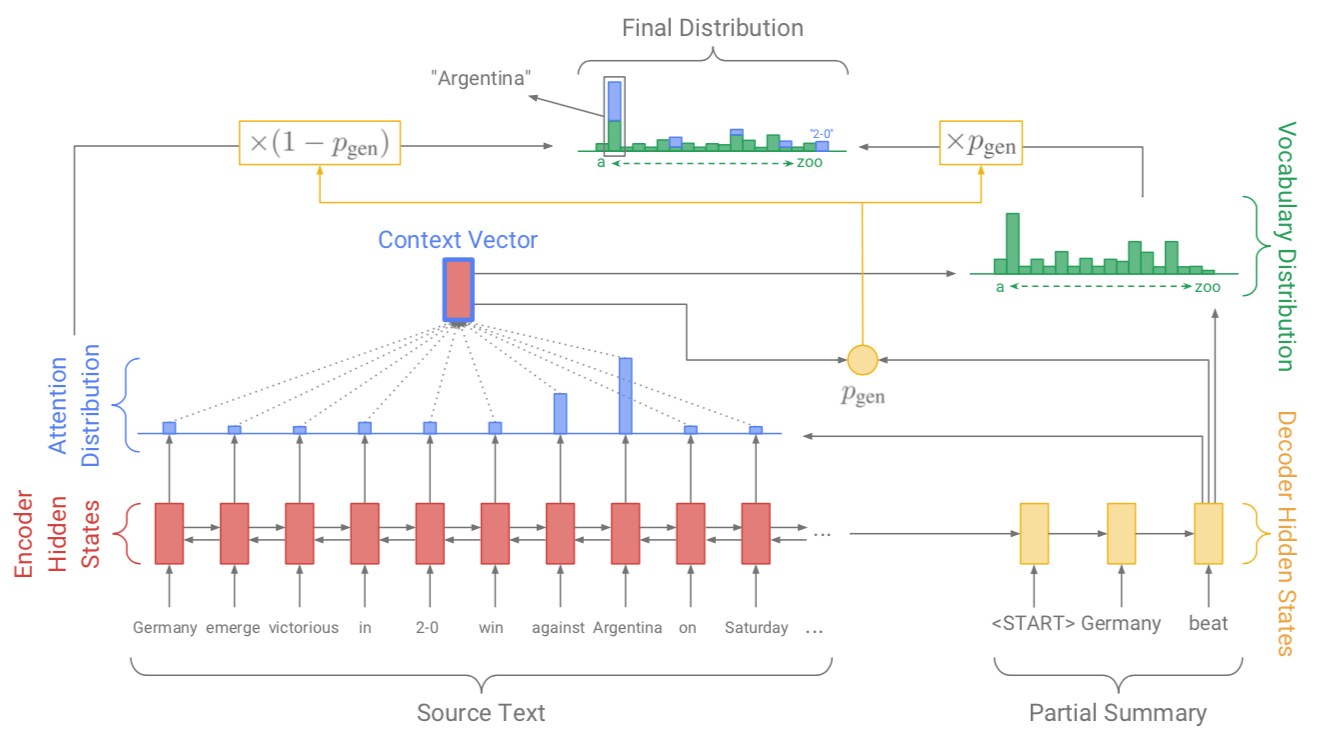
\includegraphics[width=10.0in]{./figures/SeeetalACL-17_Figure_03.png}
  \end{center}
%
        \caption{The sequence-to-sequence encoder-decoder attentional model shown here uses a specialized memory called a {\it{pointer network}} to construct a short summary of a source document by flexibly combining phrases from the source document with words from its existing vocabulary. For each decoder timestep a generation probability $P\mbox{\rm{gen}} \hmisin{} [0, 1]$ is calculated, which weights the probability of {\it{generating}} words from the vocabulary, versus {\it{copying}} words from the source text. The vocabulary distribution and the attention distribution are weighted and summed to obtain the final distribution, from which we make our prediction. Note that out-of-vocabulary article words such as "2-0" are included in the final distribution. \emdash{} adapted from See~\etal{}~\cite{SeeetalACL-17}.}
%
  \hrule{}
%
\end{figure}

%%% %%%%%%%%%%%%%%%%%%%%%%%%%%%%%%%%%%%%%%%%%%%%%%%%%%%%%%%%%%%%%%%%%%%%%%%%%%%% 

\rawhtml
<a name="automated_programming_code_repair"></a>
\endrawhtml
One approach involves representing a program as an abstract syntax tree and performing a series of repairs that involve replacing complete subtrees in the AST. It might be feasible to use some variant of the pointer-network concept, e.g., {\cite{BhoopchandetalICLR-17}}, {\cite{SeeetalACL-17}} and  {\cite{WangandJiangICLR-17}} or neural programmer framework {\cite{NeelakantanetalICLR-17}}, but there are limitations with all of the alternatives I've run across so far, requiring additional innovation to deal with the dynamic character of editing AST representations, but at least the parsing problem is solved for us \emdash{} all we have to do is make sure that our edits maintain syntactic well-formedness.

Most of the existing pointer-network applications analyze / operate on a fixed structure such as a road map, e.g., examples include the planar graphs that Oriol Vinyals addresses in his paper~\cite{VinyalsetalNIPS-15}, recognizing long-range dependencies in code repositories~\cite{BhoopchandetalICLR-17}, and annotating text to support summarization~\cite{SeeetalACL-17}. Student projects focusing on program-repair might try ingesting programs using an LSTM, creating a pointer-network / DNC-like representation of the AST and then altering selected programs by using fragments from other programs, but be advised this approach will likely require inventing extensions to existing pointer-network techniques.

One possibility for training data is to use the ETH / SRI Python {\urlh{https://www.sri.inf.ethz.ch/py150}{dataset}} that was developed by Veselin Raychev as part of his {\urlh{https://www.sri.inf.ethz.ch/raychev_thesis.pdf}{thesis}} on automated code synthesis\footnote{%
%
  From the ETH / SRI website: "We provide a dataset consisting of parsed Parsed ASTs that were used to train and evaluate the DeepSyn tool. The Python programs are collected from GitHub repositories by removing duplicate files, removing project forks (copy of another existing repository), keeping only programs that parse and have at most 30K nodes in the AST and we aim to remove obfuscated files. Furthermore, we only used repositories with permissive and non-viral licenses such as MIT, BSD and Apache. For parsing, we used the Python AST parser included in Python 2.7. We also include the parser as part of our dataset. The dataset is split into two parts \emdash{} 100K files used for training and 50K files used for evaluation."}.
%
Possible projects include designing a rewrite system for code synthesis based on NLP work from Chris Manning's lab led by Abigail See focusing on text summarization leveraging pointer networks \emdash{} see Figure~{\urlh{#fig_SeeetalACL-17_Figure_03}{2}} for a schematic description of the model from their paper~\cite{SeeetalACL-17}. Further afield are program synthesis papers that work starting from specifications like Shin~\etal{}~\cite{ShinetalICLR-18b} out of Dawn Song's lab or recent work from Rishabh Singh and his colleagues~\cite{WangetalCoRR-17}.

Another possibility is to use RL to learn repair rules that operate directly on the AST using various strategies. It's not necessary in this case to represent the AST as a pointer network, but, rather, take the expedient of simply creating a new embedding edited AST after each repair. We can generate synthetic data by taking correct programs from the ETH / SRI dataset and introducing bugs and then use these to generate a reward signal, with harder problems requiring two or three separate repairs. 

It might also be worth exploring the idea of working with program embedding vectors in a manner similar to performing arithmetic operations on word vectors in order to recover analogies \emdash{} see the analysis of Levy and Goldberg~\cite{LevyandGoldbergCONIL-14} in which they demonstrate that analogy recovery is not restricted to simple neural word embeddings. For example, given the AST for a program {\tt{P}} with subtree {\tt{Q}} and two possible repairs that correspond to replacing {\tt{Q}} with either {\tt{R}} or {\tt{R'}}, can we determine which is the better outcome {\tt{A = P - Q + R}} or {\tt{A' = P - Q + R'}} and might it serve as a distal reward signal to expedite training?

I also recommend Reed and de Freitas~\cite{ReedandDeFreitasCoRR-15} for its application of the idea of using dynamically programmable networks in which the activations of one network become the weights (program) of another network.  The authors note that this approach was mentioned in Sigma-Pi units section of Rumelhart~\etal{}~\cite{RumelhartetalPDP-86b}, appeared in Sutskever and Hinton~\cite{SutskeverandHintonNIPS-09} in the context of learning higher order symbolic relations and in Donnarumma~\etal{}~\cite{DonnarummaetalIJNS-15} as the key ingredient of an architecture for prefrontal cognitive control.

%%% %%%%%%%%%%%%%%%%%%%%%%%%%%%%%%%%%%%%%%%%%%%%%%%%%%%%%%%%%%%%%%%%%%%%%%%%%%%%

\subsubsectional{Resources}

%%% %%%%%%%%%%%%%%%%%%%%%%%%%%%%%%%%%%%%%%%%%%%%%%%%%%%%%%%%%%%%%%%%%%%%%%%%%%%% 

Michael Graziano's {\urlh{https://web.stanford.edu/class/cs379c/calendar_invited_talks/lectures/04/10/index.html}{presentation}} on machines that incorporate an internal model of what consciousness is and attribute that model to themselves and others to make predictions about human behavior~\cite{GrazianoFiRAI-17}\footnote{%
%
  The abstract for Graziano~\cite{GrazianoFiRAI-17}:
%
  \begin{quotation}
%
   The purpose of the attention schema theory is to explain how an information-processing device, the brain, arrives at the claim that it possesses a non-physical, subjective awareness, and assigns a high degree of certainty to that extraordinary claim. The theory does not address how the brain might actually possess a non-physical essence. It is not a theory that deals in the non-physical. It is about the computations that cause a machine to make a claim and to assign a high degree of certainty to the claim. The theory is offered as a possible starting point for building artificial consciousness. Given current technology, it should be possible to build a machine that contains a rich internal model of what consciousness is, attributes that property of consciousness to itself and to the people it interacts with, and uses that attribution to make predictions about human behavior. Such a machine would "believe" it is conscious and act like it is conscious, in the same sense that the human machine believes and acts.
%
  \end{quotation}}.

Randall O'Reilly's {\urlh{https://web.stanford.edu/class/cs379c/calendar_invited_talks/lectures/04/12/index.html}{presentation}} on learning mechanisms that rely on a computational model of the prefrontal cortex to control both itself and other brain areas in a strategic, task-appropriate manner~\cite{OReillyandFrankNC-06}\footnote{%
%
  The abstract for O'Reilly and Frank~\cite{OReillyandFrankNC-06}:
%
  \begin{quotation}
%
   The prefrontal cortex has long been thought to subserve both working memory (the holding of information online for processing) and executive functions (deciding how to manipulate working memory and perform processing). Although many computational models of working memory have been developed, the mechanistic basis of executive function remains elusive, often amounting to a homunculus. This article presents an attempt to deconstruct this homunculus through powerful learning mechanisms that allow a computational model of the prefrontal cortex to control both itself and other brain areas in a strategic, task-appropriate manner. These learning mechanisms are based on subcortical structures in the midbrain, basal ganglia, and amygdala, which together form an actor-critic architecture. The critic system learns which prefrontal representations are task relevant and trains the actor, which in turn provides a dynamic gating mechanism for controlling working memory updating. Computationally, the learning mechanism is designed to simultaneously solve the temporal and structural credit assignment problems.
%
  \end{quotation}}.

Jay McClelland's {\urlh{https://web.stanford.edu/class/cs379c/calendar_invited_talks/lectures/04/19/index.html}{presentation}} on complementary learning systems that avoid catastrophic forgetting and support the stable learning of new knowledge and learning with imbalanced class labels~\cite{SprechmannetalICLR-18}\footnote{%
%
  The abstract for Sprechmann~\etal{}~\cite{SprechmannetalICLR-18}:
%
  \begin{quotation}
%
   Deep neural networks have excelled on a wide range of problems, from vision to language and game playing. Neural networks very gradually incorporate information into weights as they process data, requiring very low learning rates. If the training distribution shifts, the network is slow to adapt, and when it does adapt, it typically performs badly on the training distribution before the shift. Our method, Memory-based Parameter Adaptation, stores examples in memory and then uses a context-based lookup to directly modify the weights of a neural network. Much higher learning rates can be used for this local adaptation, reneging the need for many iterations over similar data before good predictions can be made. As our method is memory-based, it alleviates several shortcomings of neural networks, such as catastrophic forgetting, fast, stable acquisition of new knowledge, learning with an imbalanced class labels, and fast learning during evaluation. We demonstrate this on a range of supervised tasks: large-scale image classification and language modeling.
%
  \end{quotation}}.

Matt Botvinick's {\urlh{https://web.stanford.edu/class/cs379c/calendar_invited_talks/lectures/04/26/index.html}{presentation}} describing a new model of reward-based learning in which a traditional dopamine system trains the prefrontal cortex to operate as its own free-standing learning system~\cite{WangetalNATURE-NEUROSCIENCE-18}\footnote{%
%
  The abstract for Wang~\etal{}~\cite{WangetalNATURE-NEUROSCIENCE-18}:
%
  \begin{quotation}
%
   Over the past 20 years, neuroscience research on reward-based learning has converged on a canonical model, under which the neurotransmitter dopamine stamps in associations between situations, actions and rewards by modulating the strength of synaptic connections between neurons. However, a growing number of recent findings have placed this standard model under strain. We now draw on recent advances in artificial intelligence to introduce a new theory of reward-based learning. Here, the dopamine system trains another part of the brain, the prefrontal cortex, to operate as its own free-standing learning system. This new perspective accommodates the findings that motivated the standard model, but also deals gracefully with a wider range of observations, providing a fresh foundation for future research.
%
  \end{quotation}}.

%%% %%%%%%%%%%%%%%%%%%%%%%%%%%%%%%%%%%%%%%%%%%%%%%%%%%%%%%%%%%%%%%%%%%%%%%%%%%%%
